% !TEX TS-program = pdfLaTeX+MakeIndex+BibTeX
% !TEX encoding = UTF-8 Unicode

\PassOptionsToPackage{unicode}{hyperref}
\PassOptionsToPackage{naturalnames}{hyperref}

\documentclass[tg]{mdtufsm}

\usepackage[T1]{fontenc}
\usepackage{fix-cm}
\usepackage{times, color}
\usepackage[utf8]{inputenc}
\usepackage{graphicx}
\usepackage{amsmath,latexsym,amssymb}
%\usepackage[hidelinks]{hyperref}
\usepackage[hidelinks,
            bookmarksopen=true,linktoc=none,colorlinks=true,
            linkcolor=black,citecolor=black,filecolor=magenta,urlcolor=blue,
            pdftitle={Exploração da Linguagem Rust para o Desenvolvimento de um Path Tracer Paralelo},
            pdfauthor={Yuri Kunde Schlesner},
            pdfsubject={Trabalho de Graduação},
            pdfkeywords={Computação Gráfica, Linguagens de Programação, Programação Paralela, Rust, Path Tracing, Informática, UFSM}
            ]{hyperref}
%\usepackage[brazilian]{babel}

%\usepackage{fontspec}
%\setmainfont{Linux Libertine G}

%%% PAGE DIMENSIONS
\usepackage[inner=30mm,outer=20mm,top=30mm,bottom=20mm]{geometry} 
\usepackage{epstopdf}
\usepackage{graphicx}
% \geometry{margin=2in} % for example, change the margins to 2 inches all round
% \geometry{landscape} % set up the page for landscape

% \usepackage[parfill]{parskip} % Activate to begin paragraphs with an empty line rather than an indent

%%% PACKAGES
%\usepackage{amsfonts}
%\usepackage{color}
%\usepackage{booktabs} % for much better looking tables
%\usepackage{array} % for better arrays (eg matrices) in maths
%\usepackage{paralist} % very flexible & customisable lists (eg. enumerate/itemize, etc.)
\usepackage{verbatim} % adds environment for commenting out blocks of text & for better verbatim
\usepackage{listings}
\usepackage{parcolumns}
%\usepackage{microtype}
%\usepackage[numbers]{natbib}
%\usepackage{subfig} % make it possible to include more than one captioned figure/table in a single float
% These packages are all incorporated in the memoir class to one degree or another...

\lstset{
	basicstyle=\scriptsize\ttfamily,
	tabsize=2,
	frame=single,
	breaklines=true,
	breakatwhitespace=true,
	xleftmargin=0cm,
	xrightmargin=0cm,
	literate=
		{á}{{\'a}}1 {é}{{\'e}}1 {í}{{\'i}}1 {ó}{{\'o}}1 {ú}{{\'u}}1
		{Á}{{\'A}}1 {É}{{\'E}}1 {Í}{{\'I}}1 {Ó}{{\'O}}1 {Ú}{{\'U}}1
		{à}{{\`a}}1 {è}{{\`e}}1 {ì}{{\`i}}1 {ò}{{\`o}}1 {ù}{{\`u}}1
		{À}{{\`A}}1 {È}{{\'E}}1 {Ì}{{\`I}}1 {Ò}{{\`O}}1 {Ù}{{\`U}}1
		{ä}{{\"a}}1 {ë}{{\"e}}1 {ï}{{\"i}}1 {ö}{{\"o}}1 {ü}{{\"u}}1
		{Ä}{{\"A}}1 {Ë}{{\"E}}1 {Ï}{{\"I}}1 {Ö}{{\"O}}1 {Ü}{{\"U}}1
		{â}{{\^a}}1 {ê}{{\^e}}1 {î}{{\^i}}1 {ô}{{\^o}}1 {û}{{\^u}}1
		{Â}{{\^A}}1 {Ê}{{\^E}}1 {Î}{{\^I}}1 {Ô}{{\^O}}1 {Û}{{\^U}}1
		{ã}{{\~a}}1 {Ã}{{\~A}}1 {õ}{{\~o}}1 {Õ}{{\~O}}1
		{ç}{{\c c}}1 {Ç}{{\c C}}1
}

% For Computer Modern:
%\def\Cpp{{C\nolinebreak[4]\hspace{-.05em}\raisebox{.4ex}{\tiny\bf ++}}}
% For Linux Libertine G
\def\Cpp{{C\nolinebreak[4]\raisebox{.20ex}{\small\bf++}}}

\newcommand{\todo}[1]{\textsf{\color{red}#1}}
\graphicspath{{./images/}}


%%=============================================================================
%% Trampa para corrigir o bug do hyperref que redefine o caption das figuras e das
%% tabelas, n�o colocando o nome ``Figura'' antes do n�mero do mesmo na lista
%%=============================================================================

\makeatletter

\long\def\@caption#1[#2]#3{%
  \expandafter\ifx\csname if@capstart\expandafter\endcsname
                  \csname iftrue\endcsname
    \global\let\@currentHref\hc@currentHref
  \else
    \hyper@makecurrent{\@captype}%
  \fi
  \@ifundefined{NR@gettitle}{%
    \def\@currentlabelname{#2}%
  }{%
    \NR@gettitle{#2}%
  }%
  \par\addcontentsline{\csname ext@#1\endcsname}{#1}{%
    \protect\numberline{\csname fnum@#1\endcsname ~-- }{\ignorespaces #2}%
  }%
  \begingroup
    \@parboxrestore
    \if@minipage
      \@setminipage
    \fi
    \normalsize
    \expandafter\ifx\csname if@capstart\expandafter\endcsname
                    \csname iftrue\endcsname
      \global\@capstartfalse
      \@makecaption{\csname fnum@#1\endcsname}{\ignorespaces#3}%
    \else
      \@makecaption{\csname fnum@#1\endcsname}{%
        \ignorespaces
        \ifHy@nesting
          \expandafter\hyper@@anchor\expandafter{\@currentHref}{#3}%
        \else
          \Hy@raisedlink{%
            \expandafter\hyper@@anchor\expandafter{%
              \@currentHref
            }{\relax}%
          }%
          #3%
        \fi
      }%
    \fi
    \par
  \endgroup
}

\makeatother

%%% END Article customizations

\title{Exploração da Linguagem Rust para o Desenvolvimento de um \emph{Path Tracer} Paralelo}
\author{Schlesner}{Yuri Kunde}
\course{Curso de Ciência da Computação}
\altcourse{Curso de Ciência da Computação}
\institute{Centro de Tecnologia}
\degree{Bacharel em Ciência da Computação}

\trabalhoNumero{}
\advisor[Profª.]{Drª.}{Charão}{Andrea Schwertner}
\orientadoratrue

\committee[Profª. Drª.]{Augustin}{Iara}{UFSM}
\committee[Prof. Dr.]{Lima}{João Vicente Ferreira}{UFSM}

\date{20}{Outubro}{2014}

\keyword{Computação Gráfica}
\keyword{Linguagens de Programação}
\keyword{Programação Paralela}
\keyword{Rust}
\keyword{Path Tracing}

%\date{} % Activate to display a given date or no date (if empty), otherwise the current date is printed

\begin{document}
\maketitle
\makeapprove

\begin{abstract}
A Computação Gráfica, e especificamente a geração de imagens por computador, é uma área com
inúmeras aplicações. No entanto, para a geração de imagens realísticas, é essencial fazer
uso eficiente do poder computacional disponível, pois é um processo que requer a realização
de um grande número de cálculos. Tradicionalmente foram utilizadas linguagens como \Cpp, que
permitem esta eficiência, para escrever estes tipos de sistemas. \emph{Rust}, uma nova
linguagem de sistemas, tem como um dos seus objetivos servir este nicho de aplicação. Este
trabalho tem como objetivo re-implementar um renderizador fotorrealista utilizando Rust,
afim de avaliar se a linguagem realmente atende as necessidades deste tipo de aplicação.
\end{abstract}

\tableofcontents

\setlength{\baselineskip}{1.5\baselineskip}

%	\item[Período de execução:] Setembro de 2014 a Dezembro de 2014
%	\item[Unidades participantes:] ~\\ Curso de Ciência da Computação \\ Departamento de Eletrônica e Computação
%	\item[Área de conhecimento:] Ciência da Computação
%	\item[Linha de Pesquisa:] Computação Gráfica, Linguagens de Programação, Programação Paralela
%	\item[Tipo de projeto:] Trabalho de Conclusão de Curso

\chapter{Introdução}

A \emph{Computação Gráfica} é a área da Ciência da Computação que estuda tópicos relacionados à
criação, análise e manipulação de imagens e conceitos relacionados. Dentre estas, a síntese (ou
renderização) de imagens é onde uma imagem é criada de forma computacional, a partir de um modelo
matemático e frequentemente buscando o fotorrealismo. Tem uma vasta quantidade de aplicações
práticas: usada na engenharia, durante o projeto de máquinas ou construções; na arquitetura, para
a visualização de espaços; para entretenimento, em efeitos especiais de filmes ou em jogos 3D e
muitas outras.

Como a geração de imagens fotorrealistas envolve essencialmente uma simulação completa da física da
luz, um processo proibitivamente lento e complexo, são utilizadas simplificações e modelos. No
passado, devido à limitada capacidade computacional disponível, eram utilizadas aproximações
grosseiras que, embora produzissem imagens atrativas, não eram muito realistas, especialmente no
quesito da aparência das superfícies e de suas interações com a luz. Com o aumento do poder
computacional disponível, vem sendo usados modelos mais fiéis à realidade e que produzem imagens
mais convincentes, algumas vezes indistinguíveis de uma fotografia real.

\emph{Path tracing} é um método de renderização que assume que a luz se comporta como uma partícula
e calcula uma imagem traçando uma série de raios pelos caminhos através quais a luz viajaria quando
refletida através de uma cena. \todo{REF} Atualmente, é um dos \todo{algoritmos mais usados} quando são demandadas
imagens com um grau de realismo extremamente alto devido à habilidade de simular o
comportamento da luz com relativa precisão. \todo{REF}

No entanto, este realismo vem ao custo de muito poder de processamento. Mesmo com o avanço
tecnológico de CPUs, a renderização de imagens continua sendo uma tarefa árdua para processadores.
Sistemas de renderização profissionais são quase exclusivamente escritos em \Cpp\ e não em
linguagens de mais alto nível, devido às penalidades de desempenho que impõem. Sistemas mais
recentes chegam a fazer o uso de GPUs para acelerar a imensa quantidade de cálculos necessária.
Tendo em vista a baixa expressividade de \Cpp\ comparada a estas outras linguagens, torna-se
interessante explorar alternativas que permitam desenvolvimento mais fácil sem sacrificar o
desempenho requerido.

A linguagem de programação \emph{Rust}, \todo{REF} um projeto de pesquisa da \emph{Mozilla Research}, tem como
seu objetivo ser uma união entre linguagens de programação de sistemas e as tidas como ``linguagens
de alto-nível'', focando simultaneamente em alto-desempenho, segurança e expressividade. Ela atinge
isso usando um modelo tradicional de compilação prévia (\emph{ahead of time}), gerando código nativo,
sem utilizar uma máquina virtual e um sistema de tipos
que permite a verificação automática dos usos de ponteiros durante a compilação, eliminando a
possibilidade de acontecerem erros de memória sem introduzir penalidades excessivas de desempenho
ou consumo de memória. Ao mesmo tempo, integra conceitos mais recentes de linguagens de programação
que aumentam sua expressividade e capacidade de facilmente descrever programas complexos.

\section{Objetivos}

\subsection{Objetivo Geral}

O objetivo geral deste trabalho é portar um \emph{path tracer} para a linguagem \emph{Rust} e, através deste processo,
realizar uma comparação quantitativa e qualitativa entre as versões escritas nesta linguagem e \Cpp, nos aspectos de
desempenho e organização de código, respectivamente. Como base será utilizado o SmallVCM \citep{smallvcm}, um
\emph{path tracer} de pesquisa escrito em \Cpp, escolhido por implementar uma variedade
de algoritmos diferentes de \emph{path tracing}, ser paralelizado utilizando \emph{multithreading} e por ser relativamente compacto, consistindo de
aproximadamente 5000 linhas de código.

\subsection{Passos de metodologia}
\begin{itemize}
	\item Estudar o código original do SmallVCM.
	\item Re-escrever uma parte do SmallVCM utilizando Rust, para a realização de
		testes.
	\item Realizar uma comparação de desempenho e expressividade de linguagem entre as duas versões,
		atentando a possíveis pontos onde a Rust pode ser melhorada.
	\item Paralelizar a nova versão do renderizador, fazendo uso das funcionalidades de Rust.
	\item Portar o restante do SmallVCM, afim de que as duas versões tenham funcionalidades
		equivalentes.
\end{itemize}

\section{Justificativa}

Rust é uma linguagem relativamente nova e, embora aplicações gráficas de alto desempenho sejam um
dos seus públicos alvo, ainda não existe uma quantidade significativa de programas deste tipo que
valide a linguagem para este propósito. A experiência e resultados adquiridos durante a realização
deste trabalho podem ajudar a guiar o desenvolvimento da linguagem para atingir este fim.

\chapter{Fundamentos e Revisão de Literatura}

Neste capítulo é dada uma descrição dos conceitos teóricos das áreas de Linguagens de Programação e de Computação Gráfica nas quais o trabalho e as ferramentas nele utilizadas, a linguagem de programação \emph{Rust} e o algoritmo de \emph{path tracing}, se baseiam.

\section{Rust}

Rust \citep{rust} é uma linguagem de programação de propósito geral, oficialmente patrocinada pela
\emph{Mozilla Research} mas desenvolvida também pela comunidade. Éla busca atender as necessidades
de programadores que atualmente utilizariam linguagens como C ou
\Cpp, por questões de desempenho ou de controle sobre o hardware. Uma de suas características mais
distintivas é o modelo de referências que utiliza, baseado em regiões \citep{tofte1997}, que
automaticamente gerencia a vida de alocações de memória, evitando com que sejam feitos erros neste
gerenciamento, ou que memória inválida seja acessada pelo programa, sem necessitar o uso de um
\emph{garbage collector}. A linguagem, originalmente projetada por Graydon Hoare como um projeto
pessoal, foi adotada pela Mozilla Research afim de servir como linguagem de
implementação do projeto Servo \citep{servo}, um browser experimental de próxima geração, mas
atualmente já cresceu além deste objetivo para se tornar um projeto maior.

Além de melhorias no gerenciamento de memória, a linguagem busca também trazer funcionalidades
tradicionalmente oferecidas em linguagens funcionais, trazendo uma forte inspiração de linguagens
como ML \citep{milner1997}. Assim, possui funcionalidades como \emph{pattern matching}, tuplas,
\emph{sum types} (também conhecidos como \emph{Algebraic Data Types} (ADTs) ou \emph{uniões
discriminadas}.) A linguagem não implementa o modelo tradicional de programação orientada a objetos,
oferecendo em troca o conceito de \emph{traits} (similares ao conceito de \emph{type classes} em
Haskell ou de \emph{interfaces} em outras linguagens) que evita alguns problemas do modelo baseado
em herança de classes, como a falta de extensibilidade de tipos e o \emph{problema diamante} em
herança múltipla \citep{scharli2003}.

O compilador oficial da linguagem, o \emph{rustc}, é implementado na própria linguagem e utiliza a
infraestrutura do projeto LLVM \citep{lattner2004}, permitindo que usufrua das capacidades de
otimização e geração de código do projeto para alcançar uma variedade de plataformas. O compilador
também tem suporte ao carregamento de \emph{plugins} durante o processo de análise, o que expõe
poderosas capacidades de meta-programação aos usuários. Alguns exemplos de projetos que utilizam
estas capacidades são o RustGPU \citep{holk2013}, que permite a compilação de código Rust para
execução paralela em GPUs, e Zinc \citep{zinc}, um \emph{framework} para desenvolvimento de
aplicações embarcadas em microprocessadores.

\subsection{\emph{Lifetimes}}

Para criar uma linguagem segura, eficiente e sem \emph{runtime}, é necessário assegurar-se que todas os ponteiros, ou referências, no programa sejam válidas quando são acessadas. Para que isto seja possível sem incidir um custo na execução, esta é uma tarefa que precisa ser feita durante a compilação do programa, e não durante sua execução, como é feito em muitas linguagens onde todos os acessos de ponteiro são testados por validez antes de serem executados.

\emph{Rust} modela esta restrição fazendo uma análise dos objetos (Tipos básicos, estruturas, referências, etc.) que tem sua vida delimitada por escopos léxicos no programa. É permitido que uma variável seja usada em escopos dentro do qual ela foi definida, e quaisquer referências criadas a esta variável tem seu tipo associado ao escopo, de forma a proibir que estas escapem para um escopo superior (onde elas não seriam mais necessariamente válidas, pois a variável teria sido destruída no fim do seu respectivo escopo.) A região na qual uma variável é válida e referências a ela podem existir é chamada de sua \emph{lifetime}.

Para suportar a mobilidade de valores para escopos mais externos, variáveis também podem ser movidas. Mover uma variável (para outra variável, para dentro de uma chamada de função ou retornando-a para fora de uma função) invalida a variável original que continha o objeto. O compilador proíbe acessos a esta variável após ela ter sido movida, pois seus conteúdos não são mais válidos. Por esta mesma razão, é proibido mover uma variável para a qual existam referências, que seriam invalidadas se isto acontecesse. Por isso, o ato de criar uma referência a partir de uma variável é chamado ``\emph{borrow}''. (``emprestar'') O direito de vida da variável é compartilhado com a referência, enquanto esta existir.

A mesma limitação de mover para fora de uma variável emprestada também limita modificações à variável original. Isto evita uma classe de problemas causados pela modificação de um objeto enquanto existam referências à objetos contidos nele. Utilizando-se um vetor redimensionável, por exemplo, poderia ocorrer uma situação em que é criada uma referência a um elemento dentro do vetor. Se forem então permitidas modificações ao vetor, este poderia ser redimensionado de forma a invalidar a referência.

Existem situações em que esta restrição de referências baseada no escopo léxico é limitada demais. Nestes casos é feito o uso de \emph{variáveis de lifetime}, que permitem que referências sejam retornadas de funções ou armazenadas em estruturas. Uma variável de \emph{lifetime} nomeada é adicionado a uma função, e pode ser usada para especificar que certas referências criadas dentro da função são válidas dentro de um escopo maior que a chamada, correspondendo invés a um escopo herdado da função que a chamou. \citep{rust-lifetimes}

\todo{Exemplos}

\subsection{Prevenção de \emph{Aliasing}}

Para facilitar a análise do comportamento de um programa pelo usuário, \emph{Rust} também impõe restrições quanto a mutabilidade de referências a objetos. Referências \emph{únicas} ou \emph{mutáveis} permitem a modificação do objeto a que apontam, mas restringem qualquer acesso a ele sem ser pela referência enquanto estiver emprestado. Referências \emph{compartilhadas} ou \emph{imutáveis} restringem a modificação do objeto para a qual apontam, mas permitem a existência de várias delas apontando para o mesmo. Isto garante que, se uma função receber uma referência compartilhada, o objeto a qual ela aponta nunca sera modificado durante a duração da função, não precisando o programador ou o compilador preocupar-se com efeitos colaterais de operações em outros objetos. Da mesma forma, se uma função receber uma função única, poderá modificá-la sem se preocupar que isto irá interferir com outros objetos ou referências presentes dentro da função. \citep{rust-lifetimes}

Esta garantia de que valores só podem ser modificados através de um único ponto por vez também automaticamente assegura que não existam erros de sincronização em programas concorrentes. Dados compartilhado por vários \emph{threads} o serão exclusivamente através de referências compartilhadas, com a garantia de que não serão modificados, e assim não precisam de exclusão mútua para evitar condições de corrida. Por outro lado, se um \emph{thread} possuir possuir uma referência única, sabe que este dado não pode ser lido em nenhum outro lugar, também evitando a necessidade de sincronismo.

\todo{exemplos}

\subsection{\emph{Traits}}

O projeto de \emph{Rust} considera importante o suporte a programação genérica sobre tipos polimór suporta o conceito de herança de classes. No entanto, ainda é essencial suportar o uso polimórfico de objetos. Este suporte é fornecido através do conceito de \emph{traits}. Um \emph{trait} é similar a uma \emph{interface}, conceito presente em várias linguagens orientadas a objeto\todo{[REF]?}: um tipo que consiste apenas de declarações de funções, sem campos de dados ou implementação, e que forma um contrato para a interação entre dois componentes do código. Estas funções devem ser posteriormente implementadas por um tipos concretos, de acordo com o contrato estabelecido, permitindo que estes tipos sejam usados de forma genérica através da interface. Um dado tipo pode implementar mais de uma interface, permitindo expor vários conjuntos de funcionalidade distintos. \todo {exemplo}

Uma vantagem de \emph{traits} sobre o modelo de herança tradicional é que se evita a ambiguidade presente em casos onde duas superclasses em de um tipo herdam de um mesmo tipo compartilhado. Isto cria uma ambiguidade onde cada classe pode conter dentro de sí uma instância separada dos campos das classes pai ou onde ambas compartilham os mesmos campos. Esta situação é chamada de ``problema diamante'', devido a estrutura do grafo de herança resultante. Por esta razão, muitas linguagens restringem seu suporte à herança simples, permitindo que classes herdem de somente uma superclasse. \todo{diagrama}

Outra vantagem é a possibilidade de se estender tipos através da definição posterior de um novo \emph{trait}. Como a implementação de um \emph{trait} para certo tipo é separada da definição do tipo em sí, pode-se fazer um tipo pré-existente suportar novas interfaces. \todo{exemplo junto com o 1o?}

\section{\emph{Path Tracing}}

\emph{Path tracing} faz parte de uma família de algoritmos comumente denominados algoritmos de
\emph{ray tracing}. Embora também utilizados na física e nas engenharias, no contexto deste trabalho
são algoritmos que tem como finalidade a produção de imagens que retratam cenas tridimensionais.

Todos os algoritmos desta família se baseiam na ideia fundamental de simular o comportamento da luz
traçando raios que saem da câmera virtual em direção à cena. Isto é o contrário do que ocorre na
vida real, onde a luz é emitida de uma fonte e viaja pelo espaço até chegar ao observador, mas não
afeta negativamente o resultado final e torna o algoritmo computacionalmente viável, pois assegura
que todo o raio traçado é um que eventualmente chegaria no observador: a maioria da luz numa cena
não chega até o observador, que subtende um espaço relativamente pequeno nela. \citep{pharr2010}

Os primeiros algoritmos deste tipo a serem usados simplesmente traçavam um raio por pixel da imagem,
encontrando a intersecção deste raio com a cena e calculando sua aparência de acordo com algum
modelo básico de iluminação. Desta forma, não eram reproduzidas sombras nem superfícies refletivas,
como espelhos ou objetos metálicos. Estes tipo de algoritmos vieram a ser chamado de algoritmos de
\emph{ray casting}.

\Citet{whitted1980} propôs um novo método que soluciona estes problemas. Além do primeiro raio
partindo da câmera, são também traçados raios que vão do ponto sendo iluminado até cada uma das
fontes luminosas, permitindo que cada luz só seja adicionada se não estiver obstruída por outro
objeto e assim permitindo a renderização de sombras. Em superfícies refletivas, outro raio é traçado
na direção do reflexo, o qual é utilizado para calcular a luminosidade naquela direção, da mesma
maneira que o raio inicial. Assim, este algoritmo implementa \emph{ray tracing recursivo}.

\Citet{cook1984} aprimoraram o algoritmo de \citeauthor{whitted1980} para que suporte uma variedade
de efeitos adicionais como superfícies foscas e translúcidas, sombras com penumbras realísticas,
profundidade de campo e borrão de movimento. Todos estes efeitos são realizados através do mesmo
método de tirar várias amostras em cada ponto da imagem, introduzindo uma variação nas direções ou
posições traçadas em cada amostra. Embora não tenha o embasamento matemático, esta é a mesma ideia
básica utilizada posteriormente em algoritmos que utilizam integração Monte Carlo.

\Citet{kajiya1986} introduz a \emph{equação de renderização}, que descreve a interação da luz com as
superfícies, modelando também a reflexão de luz em superfícies completamente foscas (ver
\autoref{fig:path_tracing}.) Esta serve como uma importante fundação teórica que é usada como base
para o cálculo da imagem ou para o desenvolvimento de aproximações. No mesmo artigo é introduzida a
técnica de \emph{path tracing}, que difere das anteriores desenvolvidas por \citeauthor{cook1984} e
\citeauthor{whitted1980} por observar que os raios mais impactantes na aparência final da imagem são
os de baixa profundidade, e assim traçando apenas um raio recursivo por amostra, evitando o
crescimento exponencial do número de raios traçados que ocorre com as outras técnicas.

Embora capaz de produzir imagens extremamente realísticas, \emph{path tracing} pode requerer uma
quantidade impraticável de amostras para renderizar satisfatoriamente certos tipos de cenas onde não
exista uma linha de visão direta entre as superfícies e as fontes de luz. Nestas cenas, a maioria da
iluminação se dá através de caminhos indiretos ou através de superfícies refratantes que projetam
padrões de luz complicados em outras superfícies (conhecidos como \emph{caustics}.) Para contornar
estes problemas foram desenvolvidas inúmeras extensões ao algoritmo de \emph{path tracing}. Dentre
elas se destaca \emph{bidirectional path tracing}, introduzido por \citet{lafortune1993}. Este
algoritmo foi depois reformulado em \citep{veach1997}, onde também foi introduzida a técnica de
\emph{multiple importance sampling} e o algoritmo \emph{Metropolis light transport}.

\begin{figure}
	\centering
	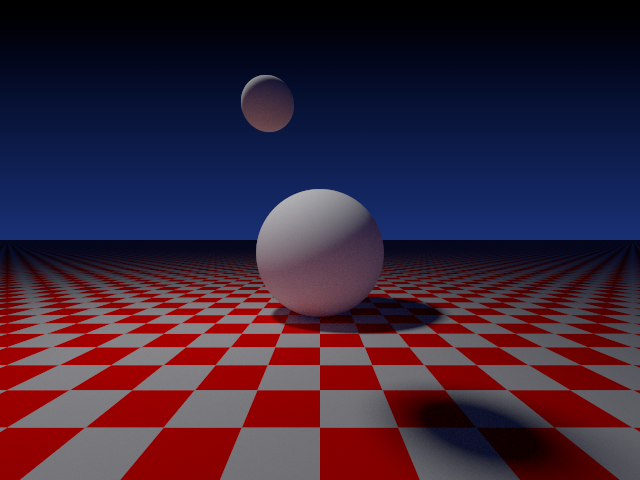
\includegraphics[width=0.5\textwidth]{exemplo_imagem}
	\caption{
		Um exemplo de uma imagem gerada utilizando \emph{path tracing}. Note como a luz que atinge o
		plano xadrez é refletida de volta para iluminar a esfera, um fenômeno conhecido como
		\emph{iluminação indireta} e que é corretamente simulado pelo algoritmo.
	}
	\label{fig:path_tracing}
\end{figure}

\section{SmallVCM}

\emph{SmallVCM} \citep{smallvcm} é um renderizador de imagens, baseado em algoritmos de \emph{ray tracing} e \emph{path tracing}, desenvolvido pelo autor para servir como uma implementação de exemplo de seu algoritmo \emph{Vertex Connection and Merging} \citep{georgiev2012}. Além deste algoritmo, o programa também implementa uma variedade de outros incluindo \emph{path tracing}, \emph{light tracing}, \emph{bidirectional path tracing} e \emph{photon mapping}. \todo{Ref. para photon mapping.} Por ter propósito de educar sobre os algoritmos, não possui funcionalidades avançadas como animação e é limitado a renderizar um pequeno conjunto de cenas de exemplo incluídas no programa. Uma imagem gerada com o programa, utilizando o algoritmo de \emph{vertex connection and merging}, pode ser vista na figura \ref{fig:smallvcm_img}. O programa também possui uma função que gera um relatório que compara a performance relativa de cada algoritmo.

\begin{figure}
	\centering
	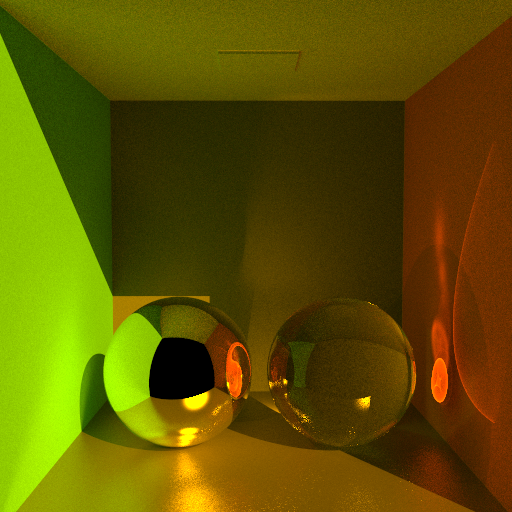
\includegraphics[width=0.5\textwidth]{ggbs_s_vcm}
	\caption{
		Uma imagem gerada pelo \emph{SmallVCM}.
	}
	\label{fig:smallvcm_img}
\end{figure}

Escrito em \Cpp, o \emph{SmallVCM} segue uma estrutura de projeto claramente organizada. A partir das opções passadas na linha de comando, é criada uma cena, utilizando um dos modelos disponíveis, e um renderizador, dos quais existem várias implementações para os vários algoritmos. Todos os renderizadores utilizam uma infra-estrutura de comum de tipos representando os objetos, fontes luminosas e materiais da cena. Os resultados intermediários da renderização são acumulados em um \texttt{Framebuffer} e subsequentemente salvos para um arquivo após um terem sido executadas um número especificado de iterações ou de certo tempo de execução.

\todo{Diagrama das classes/módulos.}

\subsection{Paralelização}

Existe suporte à paralelização do processo de renderização. Este é implementado utilizando diretivas \emph{OpenMP} \citep{openmp40}, uma API multi-plataforma para computação paralela. A \emph{OpenMP} permite a paralelização de código através da inserção de diretivas \text{\#pragma omp} em programas \Cpp, que são reconhecidas pelo compilador (portando requerendo suporte específico por parte deste) e automaticamente transformadas em código paralelo. Assim, uma aplicação existente pode ser mais facilmente convertida para um programa paralelo, sem depender de APIs de algum SO específico e sem precisar de grandes re-estruturações do programa nos casos mais simples.

No \emph{SmallVCM} a paralelização é efetuada construindo-se várias instâncias do renderizador, uma por \emph{thread}. Como cada iteração dos algoritmos de \emph{path tracing} é independente da outra, estas podem ser executadas em paralelo. Assim, pode-se atingir um determinado número de iterações em menos tempo, sem necessitar modificar os algoritmos em sí.

\chapter{Desenvolvimento}

Aqui são descritas as atividades realizadas para atingir os objetivos propostos. É dada uma explicação da organização do ambiente de compilação e desenvolvimento utilizadas nas versões do \emph{SmallVCM}. (A original e a re-escrita em \emph{Rust}, denominada \emph{SmallVCM-rs}.) Seguindo, é feita uma descrição da organização de código do \emph{SmallVCM}, e quais foram algumas diferenças marcantes encontradas entre as linguagens de como a implementação de seus componentes mudou no código \emph{Rust} por influência de diferenças entre essa linguagem e \Cpp.

\section{Ambiente de Desenvolvimento e Organização de Projeto}

\subsection{Rust}

O compilador \emph{rustc}, além de ser oficialmente distribuído em forma de código fonte, também é disponibilizado através de pacotes binários distribuídos na página do projeto\footnote{\url{http://www.rust-lang.org/install.html}}. Estes pacotes evitam que usuários passem pelo processo de \emph{bootstrap} do compilador, que pode levar mais de uma hora, dependendo do hardware em que é executado. Atualizados diariamente, os pacotes binários são providos para os sistemas operacionais Linux, Mac OS X e Windows, em versões 32-bits ou 64-bits. Ocasionalmente são também feitas versões numeradas do compilador, porém o uso destas não é recomendado pela comunidade pois rapidamente ficam defasadas, um problema se pretende-se utilizar qualquer biblioteca de terceiros ou consultar a documentação online.

Para o desenvolvimento, foi utilizada uma máquina virtual contendo o sistema operacional \emph{Arch Linux}. Além de conter software atualizado, existem pacotes de terceiros para a distribuição que automaticamente instalam versões atualizadas do compilador de Rust.\footnote{\url{https://aur.archlinux.org/packages/rust-nightly-bin/}} Como a linguagem ainda está em fase de mudança frequente, poder atualizar o compilador facilmente é importante para se manter atualizado com as últimas mudanças e funcionalidades incluídas diariamente na linguagem.

Além do compilador, também é utilizado o gerenciador de pacotes oficial \emph{Cargo}\footnote{\url{http://crates.io/}}, \todo{falar mais sobre Cargo} desenvolvido especificamente para gerenciar e compilar bibliotecas \emph{Rust}. Assim como o compilador, também existem pacotes \emph{Arch Linux} para manter este atualizado\footnote{\url{https://aur.archlinux.org/packages/cargo-nightly-bin/}}.

Seguindo sua estrutura recomendada de projeto, é possível utilizar o \emph{Cargo} para gerenciar a compilação, com o comando \texttt{cargo build}, evitando a necessidade de um \emph{Makefile}. Para fazer uso desta funcionalidade, é necessário colocar todo o código fonte dentro de um subdiretório \texttt{src/}. O ponto de partida do compilador para fazer a descoberta de todo o código fonte deve ser em um arquivo chamado \texttt{main.rs} (para projetos executáveis) ou \texttt{lib.rs} (para bibliotecas). Fora deste diretório, deve ser criado um arquivo \texttt{Cargo.toml}, que contém metadados sobre o projeto e bibliotecas utilizadas. Esta estrutura de projeto padronizada facilita a familiarização de programadores com outros projetos \emph{Rust}, já que não é necessário se adaptar a um sistema de compilação único a cada projeto.

Além das tarefas básicas de um sistema de compilação, o sistema também encarrega-se de automaticamente fazer o download e instalação de quaisquer bibliotecas externas utilizadas. Neste trabalho são utilizadas as bibliotecas \emph{time} (Biblioteca oficial para utilizar as funções de relógio do sistema operacional.) e \emph{rayon}. (Fornece uma primitiva simples para paralelização de tarefas.) Para inclusão de uma biblioteca externa, basta incluir a URL de um repositório \emph{Git} no arquivo \texttt{Cargo.toml}, e ela será automaticamente baixada e compilada antes da compilação do programa.

Para realizar o controle de mudanças foi utilizado o \emph{Git}\footnote{O repositório com o código pode ser encontrado em \url{https://github.com/yuriks/SmallVCM-rs}}, também utilizado pelo projeto original.

\subsection{C++}

O \emph{SmallVCM} original, sendo escrito em \Cpp\ precisa de um compilador para esta linguagem. Inicialmente o sistema de compilação vem configurado para utilizar-se o compilador \emph{gcc}. O processo de compilação do programa é bastante simples, bastando executar \texttt{make} para compilar o binário. Não foram necessárias nenhumas modificações a versão distribuída do código.

Foi feita uma tentativa de se utilizar o compilador \emph{clang}, que, assim como o \emph{rustc}, utiliza o \emph{LLVM} como \emph{back-end} de otimização e geração de código, a fim de tornar as comparações com a versão escrita em \emph{Rust} mais diretamente aplicáveis. Para isso, foi necessário remover o suporte a \emph{OpenMP} \todo{Cita e explicar openmp na rev. bib.} do programa, pois a tecnologia não é bem suportada pelo compilador. Esta modificação necessitou de poucas mudanças, bastando a remoção de algumas diretivas \texttt{\#include} e \texttt{\#pragma omp} e chamadas de inicialização do \emph{OpenMP}.\footnote{Esta versão pode ser encontrada em \url{https://github.com/yuriks/SmallVCM/tree/no-openmp}} Após estas modificações o programa pôde ser compilado e executado com sucesso, mas sua execução mostrou-se demorada, com o \emph{clang} gerando código menos eficiente que o \emph{gcc}. Como \emph{Rust}, assim como \emph{clang}, também utiliza o \emph{LLVM} para sua geração de código, eram esperados resultados similares, porém a versão compilada pelo \emph{clang} obteve performance muito abaixo das versões compiladas pelo \emph{gcc} e \emph{rustc}. Investigações realizadas com desenvolvedores do \emph{LLVM} em seu canal IRC indicaram que seria vantajoso tentar a última versão de desenvolvimento (\emph{Head of Tree}) do \emph{clang}, que havia recebido melhoras na geração de código em áreas relevantes ao programa. Fazendo uso da versão de desenvolvimento, constatou-se que ambos compiladores agora geravam código com desempenho similar.

\section{Metodologia da \emph{Port}}

Estabeleceu-se um objetivo inicial de converter para \emph{Rust} o conjunto de código necessário para renderizar uma imagem utilizando o algoritmo básico \emph{EyeLight}, que calcula apenas a incidência de luz direta de um fonte luminosa posicionada no observador, em modo \emph{single-threaded}. Isto possibilita que se tenha uma versão funcional para realizar testes de performance o mais cedo possível.

Procurou-se manter a organização do código da versão re-escrita em \emph{Rust} similar à do original: Os arquivos mantém o mesmo nome mas com a extensão \texttt{.cxx} ou \texttt{.hxx} substituída por \texttt{.rs}. Uma exceção é o arquivo \texttt{smallvcm.cxx}, que foi renomeado para \texttt{main.rs} para seguir a organização padronizada descrita na seção anterior.

\todo{Overview do código necessário para o objetivo.}

\section{Mudanças e Dificuldades}

Durante o processo de re-escrita foram encontradas diversas dificuldades provenientes da escolha da \emph{Rust} e de seu estado de desenvolvimento atual. Foram necessárias mudanças no paradigma de implementação de certos aspectos do programa para se adequar as convenções e funcionalidades da \emph{Rust}.

\subsection{Herança}

Um dos elementos de linguagem notoriamente ausentes de \emph{Rust} é o conceito de herança de tipos. As alternativas apresentadas para fazer re-uso de código e comportamentos polimórficos são o uso de composição e de \emph{traits}, respectivamente.

No código do \emph{SmallVCM} existem alumas instâncias de hierarquias de herança de classe, todas seguindo o mesmo padrão: Uma classe base abstrata, as vezes contendo alguns campos de dados concretos, além de definições de funções virtuais que devem ser substituídas pelas classes que as implementam. Esse padrão é utilizado pelas hierarquias definindo algoritmos de compilação (base \texttt{AbstractRenderer}); formas geométricas (base \texttt{AbstractGeometry}) e tipos de fontes luminosas (base \texttt{AbstractLight}).

Duas dessas hierarquias, de formas geométricas e de fontes luminosas, não possuem campos de dados na classe base e portanto podem ser diretamente convertidos para \emph{traits} a serem implementados por estruturas.

Para realizar a conversão da hierarquia de \texttt{AbstractRenderer}, que possui campos de dados, para Rust, adotou-se a seguinte metodologia: Como a classe base contem campos de dados, é definida uma estrutura \texttt{RendererBase}, contendo estes campos compartilhados e quaisquer funções \emph{não-virtuais} da classe base. É também definido um \emph{trait} \texttt{AbstractRenderer} contendo apenas as declarações das funções \emph{virtuais} e também adicionando duas novas funções: \texttt{base} e \texttt{base\_mut}. O propósito destas duas funções é retornar uma referência ou uma referência única, respectivamente, para uma instância \texttt{RendererBase} contida dentro do objeto, assim permitindo que código no resto do programa consiga pegar uma referência para as funções e dados da ``classe base''. As classes que originalmente derivavam de \texttt{AbstractRenderer} no código \Cpp\ agora incluem um \texttt{RendererBase} como um de seus campos e implementam o \emph{trait} para extender a estrutura/\emph{trait} base. As duas implementações são demonstradas na \todo{LISTAGEM DE CÓDIGO}.

O resultado desta conversão resulta num uso um tanto inconveniente do tipo, pois a base precisa ser explicitamente acessada quando se quer utilizar um campo, mas no geral não força nenhuma mudança arquitetural de grande porte neste caso.

\subsection{Sobrecarga de Funções}

Devido a falta de suporte a sobrecarga de funções, algumas funções tiveram que ser renomeadas durante o processo. No geral utilizou-se o mesmo nome da função original, com um sufixo indicando o tipo de parâmetro aceito pela função. Este ponto não gerou outras dificuldades.

\subsection{Sobrecarga de Operadores e Conversões Automáticas}

O módulo \texttt{math.rs} contém uma biblioteca de tipos matemáticos, consistindo de vetores 2D e 3D, além de matrizes 4x4. Este arquivo sofreu várias modificações comparado ao original devido ao seu frequente uso de sobrecarga de operadores, que diferem em sintaxe e implementação, e conversões automáticas, que não são suportadas em \emph{Rust}.

Em \emph{Rust} a sobrecarga de operadores é feita através da implementação de \emph{traits} especiais. No entanto, este é um procedimento muito mais verboso do que simplesmente declarar funções com um nome especial como é feito em \Cpp. Assim, para evitar uma grande quantidade de duplicação de código, foi usada a funcionalidade de macros de \emph{Rust} para gerar as implementações dos operadores para \texttt{Vec2} e \texttt{Vec3} sem precisar repetir todas as definições. Parte da definição desta macro e sua correspondente expansão são mostradas na figura \ref{code:mathmacro}.

\begin{figure}
\begin{lstlisting}
// Definição das macros
macro_rules! impl_Vector_op(
	($Trait:ident for $Self:ident { $($field:ident),+ }, $func:ident) => (
		impl<T: Num> $Trait<$Self<T>, $Self<T>> for $Self<T> {
			#[inline]
			fn $func(&self, o: &$Self<T>) -> $Self<T> {
				$Self {
					$($field: self.$field.$func(&o.$field)),+
				}
			}
		}
	)
)

macro_rules! impl_Vector_traits(
	($Self:ident { $($field:ident),+ }) => (
		impl_Vector_op!(Add for $Self { $($field),+ }, add)
		impl_Vector_op!(Sub for $Self { $($field),+ }, sub)
		impl_Vector_op!(Mul for $Self { $($field),+ }, mul)
		impl_Vector_op!(Div for $Self { $($field),+ }, div)

		impl<T: Num> Neg<$Self<T>> for $Self<T> {
			#[inline]
			fn neg(&self) -> $Self<T> {
				$Self {
					$($field: -self.$field),+
				}
			}
		}
		// ...
	)
)

// Definição dos tipos
#[deriving(Copy, Clone)]
pub struct Vector2<T> { pub x: T, pub y: T }
#[deriving(Copy, Clone)]
struct Vector3<T> { pub x: T, pub y: T, pub z: T }

// Instanciação das implementações utilizando macros
impl_Vector_traits!(Vector2 { x, y })
impl_Vector_traits!(Vector3 { x, y, z })
\end{lstlisting}
	\caption{Definição e uso de uma macro e sua expansão}
	\label{code:mathmacro}
\end{figure}

Outra dificuldade foi causada pela falta de conversões automáticas entre tipos. No código original ela era usada para converter escalares para vetores automaticamente, permitindo multiplicações vetor $\times$ escalar e vetor $\times$ vetor necessitando apenas de uma definição da operação de multiplicação. Para contornar isso, foram criadas funções \texttt{vec2s} e \texttt{vec3s} que realizam essa conversão. No entanto, o código usuário precisa chama-las explicitamente.

Uma alternativa seria definir um \emph{trait} \texttt{FromVector}, que poderia ser implementado por tipos escalares e vetores, convertendo os escalares para um vetor, e simplesmente retornaria o próprio vetor caso chamado nele. Esta técnica é utilizada em alguns lugares na biblioteca padrão quando é necessário realizar conversão de uma variedade de tipos diferentes de forma automática.

\subsection{Instabilidade}

\emph{Rust} ainda está em um período de intenso desenvolvimento e por isso mudanças na definição da linguagem e na implementação do compilador ainda acontecem frequentemente. Foram encontradas várias situações onde uma atualização do compilador, buscando arrumar \emph{bugs} de compilação ou tomar proveito de funções novas da linguagem, necessitou a atualização do código para se adequar a revisões feitas na linguagem.

\subsection{\emph{Enums}}

O módulo de configuração (\texttt{config.rs}) faz uso de uma \emph{enum} para selecionar o algoritmo. Em \Cpp, valores de uma enumeração tem um respectivo valor inteiro associado. \emph{Rust} não associa valores inteiros correspondentes a cada valor da enumeração, pois valores podem ter outros itens de dados associados a eles, sendo análogos a Tipos de Dados Algébricos presentes em \emph{Haskell} ou \emph{Standard ML}.  Portanto, algumas técnicas utilizadas pelo código original, como iterar através dos possíveis valores numéricos das enumerações ou as utilizar como índice em um vetor, não são possíveis aqui. Estes usos são substituídos por usos da expressão \texttt{match}, que por requerer a menção dos nomes dos itens da enumeração é mais repetitiva, mas também mais clara. Uma comparação entre os dois tipos de código pode ser vista na figura \ref{code:enums}. Nota-se que os testes para verificar se o valor está dentro do intervalo esperado não são necessários em Rust, pois a linguagem não permite a atribuição de valores não presentes na enumeração a variáveis desse tipo.

Esta funcionalidade também foi utilizada de maneira vantajosa, substituindo um par de variáveis de configuração que determinava a condição de parada do algoritmo, dos quais apenas uma poderia estar ativa de cada vez, por uma \emph{enum} de duas variantes, cada uma contendo seu respectivo parâmetro. Esta mudança evita que o sistema acidentalmente seja colocado em um estado inválido, e também remove ambiguidade na hora de testar pela condição.

\begin{figure}
	\centering
	\begin{minipage}[t]{0.48\textwidth}
\begin{lstlisting}
enum Algorithm {
	kEyeLight,
	kPathTracing,
	kLightTracing,
	kProgressivePhotonMapping,
	kBidirectionalPhotonMapping,
	kBidirectionalPathTracing,
	kVertexConnectionMerging,
	kAlgorithmMax
};

static const char* GetName(Algorithm aAlgorithm) {
	static const char* algorithmNames[7] = {
		"eye light",
		"path tracing",
		"light tracing",
		"progressive photon mapping",
		"bidirectional photon mapping",
		"bidirectional path tracing",
		"vertex connection and merging"
	};

	if(aAlgorithm < 0 || aAlgorithm > 7)
		return "unknown algorithm";

	return algorithmNames[aAlgorithm];
}

static const char* GetAcronym(Algorithm aAlgorithm) {
	static const char* algorithmNames[7] = {
		"el", "pt", "lt", "ppm", "bpm", "bpt", "vcm" };

	if(aAlgorithm < 0 || aAlgorithm > 7)
		return "unknown";
	return algorithmNames[aAlgorithm];
}
\end{lstlisting}
	\end{minipage}
	~
	\begin{minipage}[t]{0.48\textwidth}
\begin{lstlisting}
enum Algorithm {
	EyeLight,
	PathTracing,
	LightTracing,
	ProgressivePhotonMapping,
	BidirectionalPhotonMapping,
	BidirectionalPathTracing,
	VertexConnectionMerging,
}

impl Algorithm {
	fn get_name(self) -> &'static str {
		match self {
			EyeLight => "eye light",
			PathTracing => "path tracing",
			LightTracing => "light tracing",
			ProgressivePhotonMapping => "progressive photon mapping",
			BidirectionalPhotonMapping => "bidirectional photon mapping",
			BidirectionalPathTracing => "bidirectional path tracing",
			VertexConnectionMerging => "vertex connection and merging",
		}
	}

	fn get_acronym(self) -> &'static str {
		match self {
			EyeLight => "el",
			PathTracing => "pt",
			LightTracing => "lt",
			ProgressivePhotonMapping => "ppm",
			BidirectionalPhotonMapping => "bpm",
			BidirectionalPathTracing => "bpt",
			VertexConnectionMerging => "vcm",
		}
	}
}
\end{lstlisting}
	\end{minipage}
	\todo{sub-captions}
	\caption{Comparação entre \emph{enums} em C++ e \emph{Rust}}
	\label{code:enums}
\end{figure}

\subsection{Ponteiros Nulos}

\emph{Rust} desestimula o uso de ponteiros, \todo{rev bib: restringindo seu uso a blocos especiais utilizados para a escrita de código baixo nível livre da checagem estática de segurança de memória.} Programadores devem geralmente substituí-los por referências, que não podem ser nulas e que também estão são verificadas em compilação para garantir que nunca se tornem inválidas, ou utilizar o tipo `Box<T>`, que representa uma alocação de memória pertencente a uma variável ou campo e que é gerenciada automaticamente para manter estas mesmas garantias.

O código original inicializava alguns ponteiros para nulo. Em sua maioria estes casos foram simplesmente adaptados para diretamente inicializar o ponteiro com seu valor final, agora com a garantia de que sempre terão um valor válido. Em um caso foi utilizado o tipo \texttt{Option<T>}, \todo{explicar option na rev. bib.} para permitir uma alocação opcional de um valor. Este uso também poderia ser eliminado com alguma re-estruturação do código.

\subsection{Biblioteca padrão}

\todo{TODO}

\todo{Para a leitura de parâmetros passado via linha de comando, é utilizada o módulo \texttt{getopts} presente na biblioteca padrão. Na versão \Cpp\ a leitura é feita de forma manual.}

\chapter{Próximas Etapas}

\todo{Como continuação do trabalho realizado até o momento, são planejadas as seguintes atividades:}

\begin{enumerate}
	\item Continuar a re-escrita em andamento do SmallVCM, afim de que esta tenha funcionalidade o suficiente para gerar imagens usando pelo menos um tipo de algoritmo.
	\item Paralelizar o código do renderizador, explorando diferentes alternativas para atingir este fim.
	\item Realizar testes comparativos para determinar o desempenho relativo entre duas versões, como parte do objetivo de determinar se a linguagem \emph{Rust} é compatível com este tipo de aplicação.
	\item Trazer o resto dos algoritmos de renderização do SmallVCM à versão em \emph{Rust}, para que ambos tenham o mesmo conjunto de funções.
\end{enumerate}

\setlength{\baselineskip}{\baselineskip}
\bibliographystyle{abnt}
\bibliography{../graphics,../languages}

\end{document}
